
\documentclass[11pt]{amsbook}

\usepackage{../HBSuerDemir}	% ------------------------


\begin{document}

% ++++++++++++++++++++++++++++++++++++++
\hPage{b2p2/266}
% ++++++++++++++++++++++++++++++++++++++
	
	\par A function of two variables may also be defined implicitly as $F(x, y, z)=0$ (by a restrictor). Unless otherwise stated it is considered that $z$ is the dependent variable. However $F(x, y, z)=0$ may define $x$ (or $y$) as a function of the other two variables.
	\begin{exmp}
		Which ones of the following relations are functions. If not, write a restriction to be a function.
			\begin{enumerate}[label=\alph*)]
				\begin{multicols}{2}	
				\item $ x^2+y^2+z^2=16 $
				\item $x^2+y-z^2=0 $
				\end{multicols}
				\begin{multicols}{2}
				\item $ -2z = 2x^2+y^2$
				\item $z^3=x$
				\end{multicols}
			\end{enumerate}
			
			\begin{hSolution}
	
				\begin{enumerate}[label=\alph*)]
					
					\item This relation is not a function, since $P(x, y)$ has more than one image. A restriction for this to be a function is $z>0$. Another restriction is, for instance, the point $(0, \sqrt{7}, -3)$ lies on the surface.
					\item Same as in (a), A restriction is $z>5$. Observe that $y$ is a function of $x$ and $z$.
					\item This is a function, since to each pair $(x, y)$ there is assigned a single image, namely $z=-x^2-^2/2$.
					\item It is a function: $z= f(x, y) = \sqrt[3]{x}$.
				\end{enumerate}
			\end{hSolution}

	\end{exmp}
	\begin{exmp}
		Find and sketch the domains of the following functions:
			\begin{enumerate}[label=\alph*)]
				\begin{multicols}{2}	
				\item $z=e^{xy} $
				\item $z=\ln{xy}$
				\end{multicols}
				\begin{multicols}{2}
				\item $ z=\sqrt{1-x^2-y^2}$
				\item $z=\frac{e^x}{1-y}$
				\end{multicols}
			\end{enumerate}
			\begin{hSolution}
				\begin{enumerate}[label=\alph*)]
				\begin{multicols}{2}	
				\item $ D=R^2 $ 	 ~\\			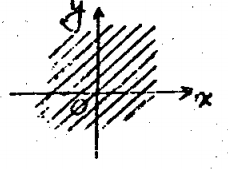
\includegraphics[width=0.2\textwidth]{images/b2p2-266-fig01}
				\item $D={(x, y): xy>0} $	 ~\\		 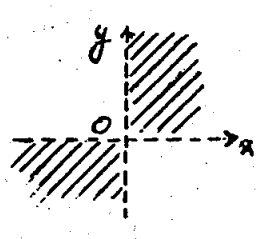
\includegraphics[width=0.2\textwidth]{images/b2p2-266-fig02}
				\end{multicols}
			\end{enumerate}
			\end{hSolution}
	\end{exmp}

% =======================================================
\end{document}  

